\documentclass[a4paper,titlepage]{report}

\usepackage{graphicx}
\usepackage{amssymb}

\begin{document}

\begin{titlepage}

\begin{center}
 
\Large\textbf{Department of Physics and Astronomy\\
University of Heidelberg}

\vspace{18cm}

\normalsize
Bachelor Thesis in Physics\\
submitted by\\
\vspace{0.5cm}
\Large\textbf{Maximilian Argus}\\
\normalsize
\vspace{0.5cm}

born in Hamburg, Germany\\
\vspace{0.5cm}
\Large\textbf{1990}
\normalsize

\newpage




\Large\textbf{Electric Field Optimization of a Rydberg Atom Experiment}

\vspace{18cm}

\normalsize
This Bachelor Thesis has been carried out by Maximilian Argus at the\\
Physikalisches Institute in Heidelberg\\
under the supervision of\\
Prof. Dr. Matthias Weidem\"uller

\vfill
\end{center}

\end{titlepage}


\begin{abstract}
Modern experiments with ultracold Rydberg atoms with application to
many body physics and quantum information science, demand a high
level of experimental sophistication to precisely control experimental
parameters like external electric fields, as Rydberg atoms are very
 polarizable. In the experiment this is achieved by (a structure hosting)
>10 individually controllable electrodes. However, the task of finding
the optimal control voltages for these is complicated by incomplete
knowledge of the charge distributions, including possible patch fields
(making it particularly time consuming). To overcome this challenge
we have applied evolutionary algorithms, a group of powerful search
heuristics, to optimize the overall performance of our experiment. With
particular focus on electric field control we asses the performance of
several algorithms, on competing requirements of noise robustness and
fast convergence, in solving two problems: cancellation of electric fields
and and optimum guiding of field ionized Rydberg atoms to a MCP
detector. Additionally Foreseeable applications to controlling quantum
state evolution and engineering strongly correlated many body systems
of interacting Rydberg atoms will be considered.
\end{abstract}



\section*{Introduction}
Introduction introduction introduction

\tableofcontents

\chapter{Concept}


\chapter{Theoretical Background}

\chapter{Mathematical Optimization}

A $n$ dimensional real value optimization problem can be stated in the form
\[ min f(\mathbf{x})  \]
for
\[ f: S \rightarrow  \mathbb{R} \]
where
\[ \mathbf{x} \in S  \subseteq \mathbb{R}^n \]

\noindent
A point $\mathbf{x}^* \in D$ is a global minimum if  $ f(\mathbf{x}^*) \leq f(\mathbf{x}^*)  \forall  \mathbf{x} \in S$

\noindent
A point $\mathbf{x}^* \in D$ is a local minimum if  in the surrounding  $ U \subseteq S$ of  $\mathbf{x}^*$ it holds that $f(\mathbf{x}^*)  \leq f(\mathbf{x})  \forall  \mathbf{x} \in U$

As there are many different types of optimization algorithms only the subset of Monte Carlo probablistic global optimization algorithms will be considered. These algorithms sacrifice both evaluating the entire search space and evaluating the function exactly, in favour of a shorter runtime. In these algorithms the choice of which candidates to evaluate is made by a heuristic which makes an induction based on previous evaluations. A suitable choice of heuristic is dependent on the problem being optimized.  A futher subset of heuristics is Evolutionary Computation, this method maintains a set of possible solution candidates which it tries to refine over a number of generations.



\newpage
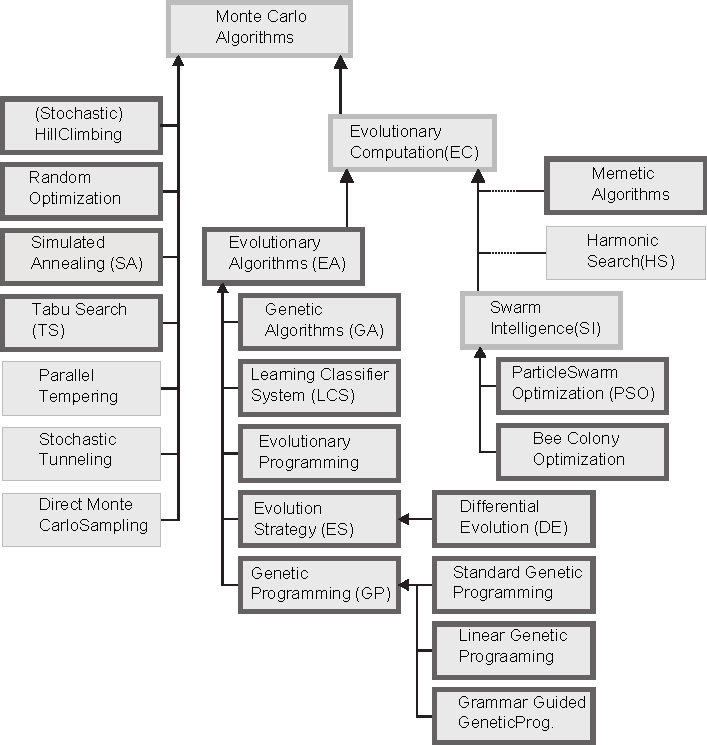
\includegraphics{Images/taxonomy_v2.pdf}



\end{document}